\documentclass[a4paper, 10pt]{article}
\usepackage{helvet}
\renewcommand{\familydefault}{\sfdefault}
\usepackage{pgf}
\usepackage{eurosym}
\usepackage{graphicx}
\usepackage{wasysym}
\usepackage{hyperref}
\usepackage{listings}
\usepackage{pxfonts}
\usepackage{verbatim}
\usepackage{color}
\usepackage{xcolor}
\usepackage{wrapfig}
\usepackage{enumitem}
\usepackage{booktabs}
\usepackage{gensymb}
\usepackage{tabularx}
\usepackage{currfile}

\hypersetup{
    bookmarks=true,         % show bookmarks bar?
    unicode=true,          % non-Latin characters in Acrobat’s bookmarks
    pdftoolbar=true,        % show Acrobat’s toolbar?
    pdfmenubar=true,        % show Acrobat’s menu?
    pdffitwindow=true,     % window fit to page when opened
    pdftitle={Assessments},    % title
    pdfauthor={Paul Vesey},     % author
    pdfsubject={I.C.T. Building Information Modelling},   % subject of the document
    pdfcreator={},   % creator of the document
    pdfproducer={xelatex}, % producer of the document
    pdfkeywords={'Graphics' }, % list of keywords
    pdfnewwindow=true,      % links in new PDF window
    colorlinks=true,       % false: boxed links; true: colored links
    linkcolor=violet,          % color of internal links (change box color with linkbordercolor)
    citecolor=magenta,        % color of links to bibliography
    filecolor=red,      % color of file links
    urlcolor=blue           % color of external links
}

\setlength\parindent{0pt}
\begin{document}

\lstset{language=HTML,
				basicstyle=\small,
				breaklines=true,
        numbers=left,
        numberstyle=\tiny,
        showstringspaces=false,
        aboveskip=-20pt,
        frame=leftline
        }
				
\begin{figure}
	\centering
	
\includegraphics[width=0.5\linewidth]{./Assignments/img/LITlogo}
\end{figure}


\begin{tabularx}{\textwidth}{ |l|X| }
	\hline
	\textbf{Subject:} & COMP06051-ICT \& BIM\\
	\textbf{Course:} & BEng in Civil Engineering\\
	\textbf{Session:} & Autumn 2022\\
	\textbf{Lecturer:} & Paul Vesey \footnotesize{BEng, MIE, HDip}\\
	\textbf{Filename:} & \currfilebase\\
	\hline
\end{tabularx}



\vspace{0.25cm}	
	
\begin{flushleft}
\Large\textbf{Assignment 1 (25\% of 40\%) Microsoft PowerApp}\\
\end{flushleft}

In this assignment you will create a 3 Screen Mobile Phone app using Microsoft PowerApps.  The key deliverables for this project are:

\begin{enumerate}
	\item 3 Screen Microsoft PowerApp
	\item Connection to Microsoft Excel Data Store
	\item Share and Deployment to your lecturer's profile (paul.vesey@lit.ie) 
\end{enumerate}

\textbf{General Scope}\\


You have been provided with three screen designs as shown in Figures \ref{fig:homescreen}, \ref{fig:inputscreen} and \ref{fig:confirmationscreen}.  You are required to convert these screen designs into a working mobile phone app, using the Microsoft PowerApps tools available through your Office 365 profile.

\vspace{0.5cm}

\begin{figure}[th]
	\centering
	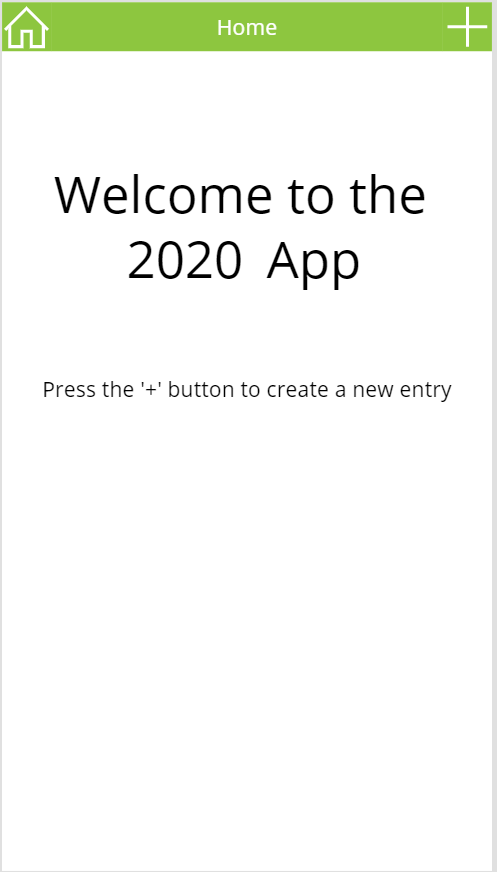
\includegraphics[width=0.7\linewidth]{img/HomeScreen}
	\caption[HomeScreen]{HomeScreen}
	\label{fig:homescreen}
\end{figure}


\begin{figure}[th]
	\centering
	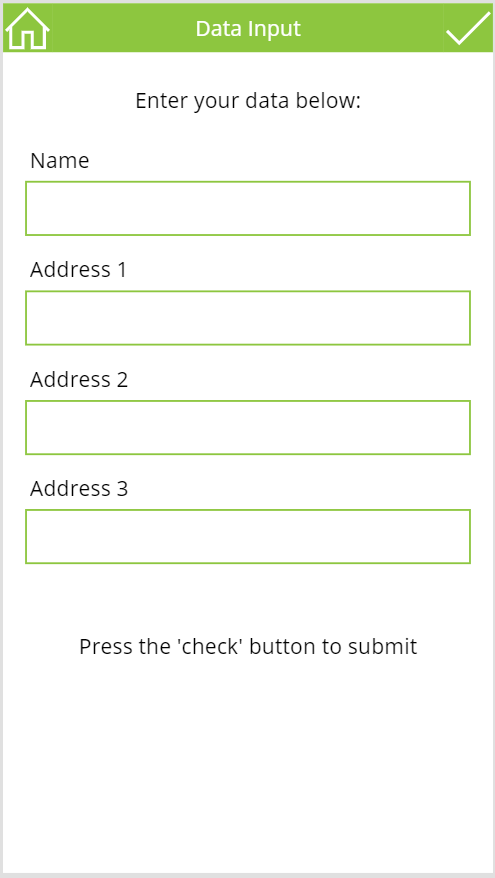
\includegraphics[width=0.7\linewidth]{img/InputScreen}
	\caption[InputScreen]{InputScreen}
	\label{fig:inputscreen}
\end{figure}


\begin{figure}[th]
	\centering
	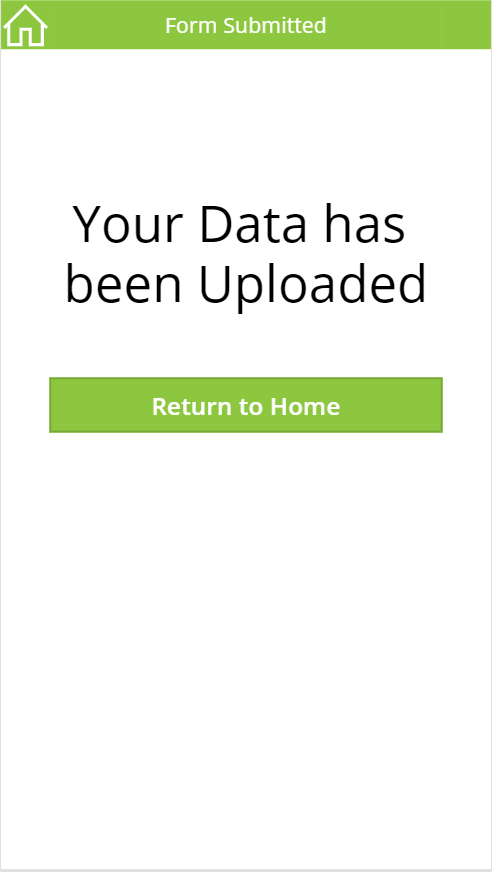
\includegraphics[width=0.7\linewidth]{img/ConfirmationScreen}
	\caption[ConfirmationScreen]{ConfirmationScreen}
	\label{fig:confirmationscreen}
\end{figure}




\vspace{.5cm}

\textbf{Suggested Approach}

\begin{itemize}
	\item Create the screens as shown in the design images, with the exception of the InputForm on the InputScreen
	\item Create the Navigation between the screens as necessary
	\item Create your Excel spreadsheet, and associated Table on OneDrive for Business, complete with all necessary column headings
	\item Create a connection from your PowerApp to your OneDrive for Business.  Complete the connection to your Excel Spreadsheet
	\item Ensure your application can create a NewForm and that the SubmitForm functionality is working correctly
	\item Conduct several test to ensure the application behaves as designed.
\end{itemize}


\newpage


\textbf{Submission}\\
This project will be completed on Microsoft PowerApps and Office 365. As such, the submission will be live documents.  All work on the platform must be completed before the date and time specified on Moodle.  Key components of the submission are:
\begin{itemize}
	\item Completed Microsoft PowerApp; make paul.vesey@lit.ie a Co-Owner
	\item Completed Microsoft Excel spreadsheet: share to paul.vesey@lit.ie
\end{itemize}

\vspace{0.5cm}
\textbf{Late Submission}\\
Failure to submit your assignment on or before the date and time indicated on Moodle will result in a penalty of 5\% per day or part thereof.

\vspace{0.5cm}
\textbf{Marking Scheme}

\begin{table}[h!]
     \begin{center}
     \begin{tabular}{p{8cm}  p{2cm} }
     \toprule
      \textbf\large{Element} & \textbf\large{Proportion} \\ 
    \cmidrule(r){1-1}\cmidrule(lr){2-2}
      \textbf{Working Mobile Phone PowerApp} & \textbf{80\%}\\
      \textbf{Excel Spreadsheet for Data Store} & \textbf{20\%}\\
      \\ \bottomrule
      \end{tabular}
      \label{tbl:markSchemeAsmt3}
      \end{center}
 \end{table}


\end{document}